\section{Recursive neural network models} \label{methods}

We study neural models that adhere to the linguistic \ii{principle of
  compositionality}, which says that the meanings for complex
expressions are derived from the meanings of their constituent parts
via specific combination functions \cite{Partee84,Janssen97}. In our
distributional model, word meanings are vectors of length $N$. The
combination function concatenates pairs of them to form vectors of
length $2N$ and maps those larger vectors back into length $N$
vectors, which can then be merged again to create more complex
phrases. Once the entire sentence-level representation has been
derived, it fed to a classifier trained in a supervised manner.

% The models that we study are centered around a recursively applied composition function which is meant to mimic the recursive construction of meanings in formal semantics. In this scheme, pairs of words are merged into phrase representations by a function that maps from representations of length $2N$ to representations of length $N$. These phrase representations are then further merged with other words and phrases until the entire phrase or sentence being evaluated is represented in a single vector. This vector is then used as the input to a classifier and used in a supervised learning task.

We use the model architecture proposed in \cite{bowman2013can} and
depicted in Figure~\ref{sample-figure}. The two phrases being compared
are built up separately on each side of the tree, using the same
composition function, until they have each been reduced to single
vectors. The resulting vectors are fed into a separate comparison
layer that is meant to generate a feature vector capturing the
relation between the two phrases. The output of this layer is then
given to a softmax classifier, which in turn produces a hypothesized
distribution over the seven relations represented in Table~\ref{b-table}.

For a composition layer, we evaluate models with both the plain neural
network layer function (eq.~\ref{rnn}) and the RNTN layer function
proposed in \citet{chen2013learning} (eq.~\ref{rntn}). A sigmoid
nonlinearity (element-wise $\tanh$) is applied to the output of either
layer function, following \cite{socher2013acl1}.
%
\begin{gather} \label{rnn}
y_{\textit{RNN}} = f(\mathbf{M} [\vec{x}^{(l)}; \vec{x}^{(r)}] + b_i)\\ % TODO: Add column vectors?
\label{rntn}
y_{\textit{RNTN}} = f(\vec{x}^{(l)T} \mathbf{A}^{[1 \ldots N]} \vec{x}^{(r)} + \mathbf{B} [\vec{x}^{(l)}; \vec{x}^{(r)}] + \vec{c})
\end{gather} % TODO: Explain third order tensor parameter?
%
Here, the $l$ and $r$ superscripts indicate the vector representations
for the left and right children of the local structure interpreted as
$y$. The RNN concatenates them, multiplies them by an $N \times 2N$
matrix of learned weights, and applies the element-wise non-linearity
to the resulting vector (plus a bias term). The RNTN has the same
basic structure, but with the addition of a tensor $\mathbf{A}$,
dimension $2N \times N \times N$, modeling interactions between the
child vectors.

The comparison layer uses the same type function template as the
composition function (either an NN layer or an NTN layer) with
independantly learned parameters and a separate nonlinearity function.
Rather than use a $\tanh$ nonlinearity here, we found a substantial
improvement in performance by using a rectified linear function for
$f_{b}$. In particular, we use the leaky rectified linear function
\cite{maasrectifier}: $f_{b}(\vec{x})=\max(\vec{x}, 0) +
0.01\min(\vec{x}, 0)$, applied element-wise.

To run the model forward and label a pair of phrases, the structure of
the lower layers of the network is assembled so as to mirror the tree
structures provided for each phrase. The word vectors are then looked
up from the vocabulary matrix $V$ (one of the model parameters), and
the composition and comparison functions are used to pass information
up the tree and into the classifier at the top. For an objective
function, we use the negative log of the probability assigned to the
correct label.

We train the model with minibatch stochastic gradient descent (SGD)
with learning rates computed using AdaGrad \cite{duchi2011adaptive}
from a starting rate of 0.2. The parameters (including the vocabulary)
are initialized randomly using a uniform distribution over $[-0.1,
0.1]$. % TODO: Update
Source code and generated data will be released after the conclusion
of the review period.

\begin{figure}[htp]
  \centering
  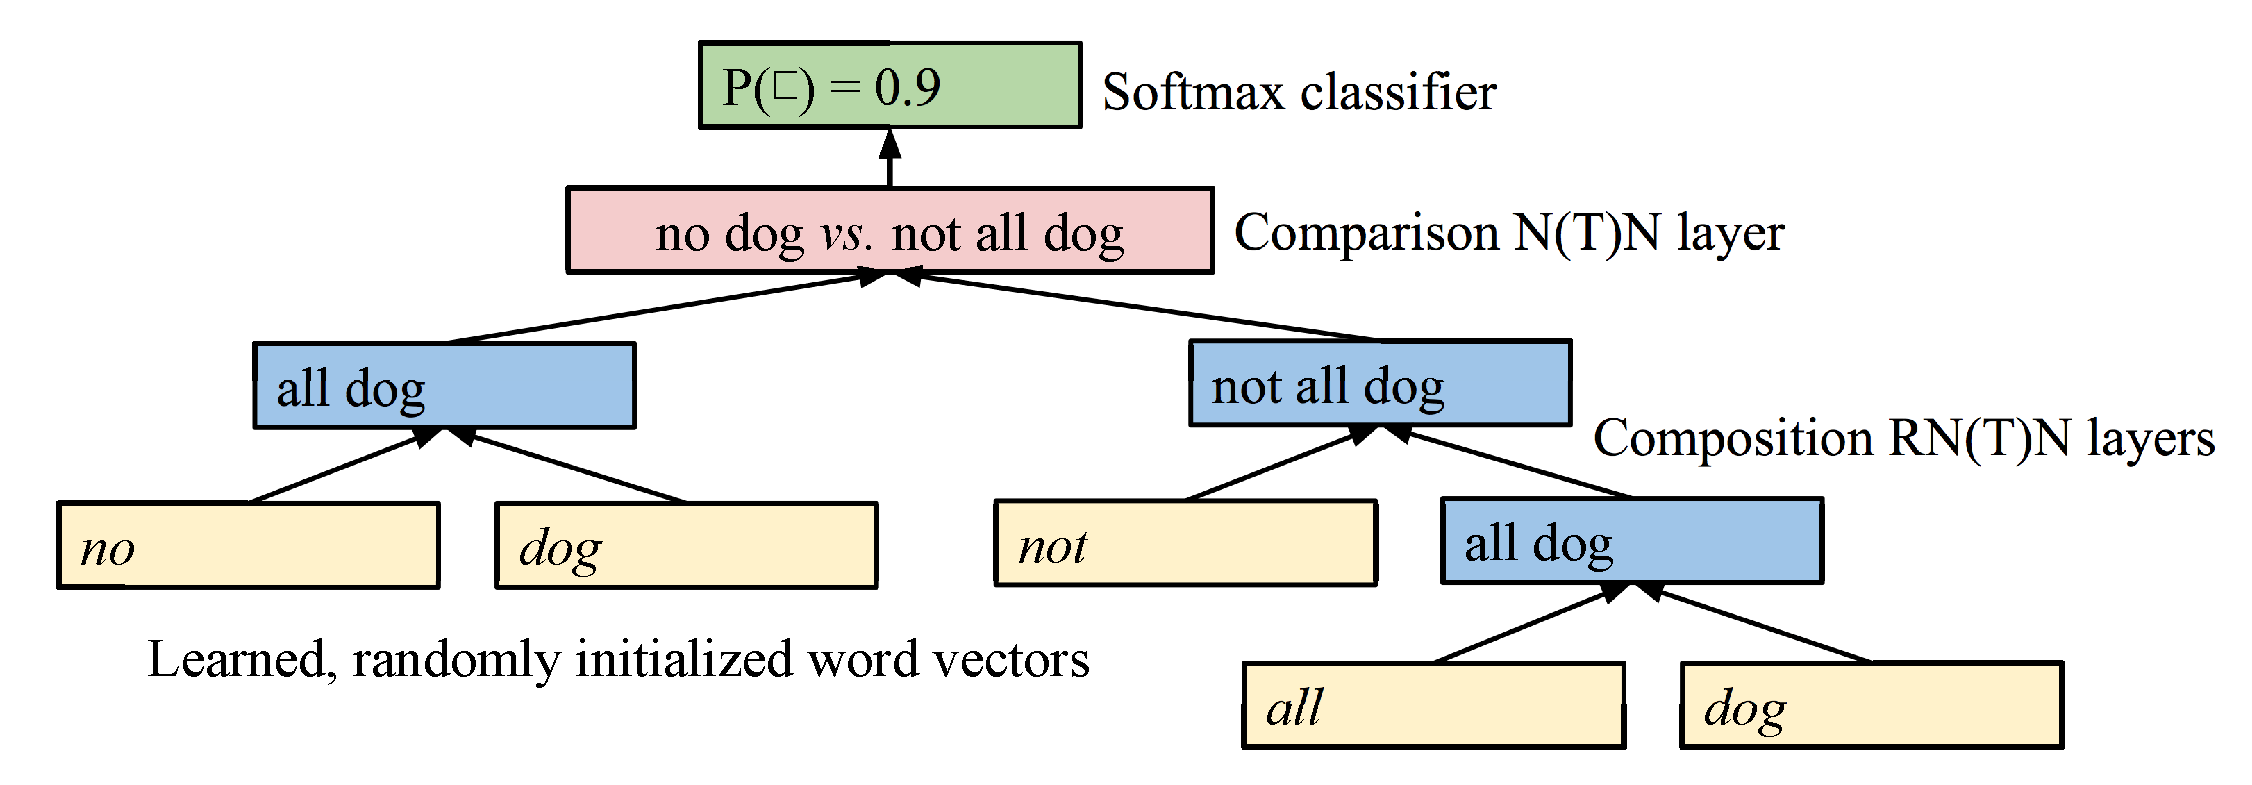
\includegraphics[scale=0.35]{model.eps}
  \caption{The model structure used to compare \ii{no dog} and \ii{(not all) dog}. 
    The same structure is used for both the RNN and RNTN layer functions.} 
  \label{sample-figure}
\end{figure}

%\ii{Source code and generated data will be released after the conclusion of the review period.} % TODO: Or upon request? Attach anonymized code?

